\section{Aufbau und Durchführung}\label{sec:AufbauDurchfuehrung}

Im folgenden wird zunächst der Aufbau der Messvorrichtung anhand der schematischen Darstellung in Abbildung \ref{fig:detektor} erläutert und anschließend die Durchführung des Experiments beschrieben.

\subsection{Aufbau}\label{subsec:Aufbau}
Eine schematische Darstellung des in dem Experiment verwendeten Aufbau des Detektors ist in Abbildung \ref{fig:detektor} zu sehen.
Über eine Hochspannungsquelle werden zwei Photomultiplier betrieben, die sich an zwei gegenüberliegenden Seiten eines mit einem organischem Szintillator gefüllten Stahlzylinders befinden.
Bewegt sich ein Teilchen durch das Szintillatormaterial, werden die Elektronen in den Atomhüllen des Szintillators durch die Wechselwirkung zwischen den Myonen und den Atomen angeregt und emittieren beim Rückgang in den Grundzustand Photonen.
Diese Photonen bewegen sich radialsymmetrisch um die Flugbahn des Myons aus, wodurch einige das Fenster des Photomultipliers erreichen, wo sie jeweils ein Elektron aus seiner Bindung durch den Photoeffekt herauslösen.
Das Elektron wird beschleunigt, schlägt dabei weitere Elektronen aus und es entsteht eine Lawine, die als negativer Spannungspuls hinter den Photomultipliern mithilfe eines Oszilloskopes aufgezeichnet werden können.
Zerfällt ein Myon in ein Elektron, dann ist auch das Elektron in der Lage den Szintillator zum emittieren von Photonen anzuregen. \newline
Bevor die Signale der Photomultiplier weiterverarbeitet werden, werden sie mithilfe von Verzögerungsleitungen synchronisiert.
Die Signale der Photomultiplier wird mithilfe eines Diskriminators slektiert, was bedeutet dass der Untergrund mithilfe einer \textit{threshold}-Spannung unterdrückt wird.
Übersteigt ein Signal den vorgegebenen Schwellwert, wird ein Rechteckimpuls erzeugt, der sich meist im sogenannten \textit{NIM-Standard} befindet. % (siehe \autoref{subsec:NIM-Standard}).
\textit{NIM} steht für \textit{Nuclear Instrument Module} und ist ein Standard für die Verarbeitung von Signalen in der Kernphysik.
Es legt Kabel und Stecker fest, die in der Kernphysik verwendet werden, um die Verbindung von Geräten zu standardisieren und somit Kompatibilität und ein schnelle Verarbeitung von Signalen zu gewährleisten.
Außerdem wird die Gleichzeitigkeit an logischen-\textit{AND}-Gattern dadurch besser definiert.
Ein Signal, das unter dem Schwellwert liegt wird nicht weiter betrachtet und somit herausgefiltert.
Durch die Diskretisierung in Rechteckspannungen, eignen sie sich bereits als digitale Signale.\newline
Die Signale aus den beiden Diskriminatoren werden in einen Koinzidenzschaltkreis geleitet, der die Signale beider Photomultiplier miteinander vergleicht.
Es wird nur ein Signal weitergeleitet, wenn beide Signale gleichzeitig auftreten, weshalb die vorgeschaltete Verzögerung notwendig ist, da somit Unterschiede in der Geschwindigkeit der Signalweiterverarbeitung zwischen den beiden Photomultipliern ausgeglichen werden kann.
Dieser Schritt filtert weiteren Untergrund aus den Messwerten heraus.\newline
Nun wird das Signal aus dem Koinzidenzschaltkreis in drei Wege aufgeteilt, wobei zwei davon sofort an verschiedene AND-Gatter weitergeleitet werden.
AND-Gatter sind logische Schaltungen, die nur dann ein Signal weiterleiten, wenn beide Eingangssignale gleichzeitig auftreten.
Das dritte Signal wird an eine weitere Verzögerungskomponente weitergeleitet, die das Signal um feste $\SI{30}{\nano\second}$ verzögert.
Nach der Verzögerungskomponente wird ein Monoflop geschaltet, der das gepulste Signal in ein durchgängiges binäres Signal umwandelt.
Der Monoflop gibt ein negiertes und ein normales Signal aus, die an die beiden AND-Gatter weitergeleitet werden.
Somit ist das erste AND-Gatter ein \textit{Veto}-Gatter, das nur dann ein Signal weiterleitet, wenn das Signal des Monoflops negiert ist, also genau dann, wenn kein Signal am Monoflop eingetroffen ist und es noch nicht zurück in seinen Grundzustand (ein Signal am negierten Anschluss) zurückgefallen ist.
Das zweite AND-Gatter leitet das Signal nur dann weiter, wenn das Signal am Monoflop auftritt, was durch die Verzögerungskomponente erst nach $\SI{30}{\nano\second}$ geschieht.
Somit können die Signale der beiden Gatter für das Starten und Stoppen einer \textit{time-amplitude-converter}-Schaltung verwendet werden, die die Zeitdifferenz zwischen den beiden Signalen misst.
Ohne die Verzögerung würde das Startsignal ebenfalls das Soppsignal sein.
In dem Versuch stellt das Startsignal das Eintreten eines Myons in den Detektor dar.
Das Stoppsignal entspricht dem Zerfall eines Myons in diesem, wodurch letzlich die mittlere Lebensdauer von kosmischen Myonen bestimmt werden kann. \newline
Die TAC wird an einen PC angeschlossen, der mithilfe eines Multi-Channel-Analysers (MCA) die Signale aufnimmt.
Ein MCA ist ein Gerät, das die Signale in einem bestimmten Zeitfenster aufnimmt und in einem Histogramm darstellt.
Meist wird ein schneller Analog-Digital-Wandler (ADC; kurz für \textit{Analog-Digital-Converter}) verwendet, um die Signale aufzunehmen und zu speichern.
\begin{figure}[H]
    \centering
    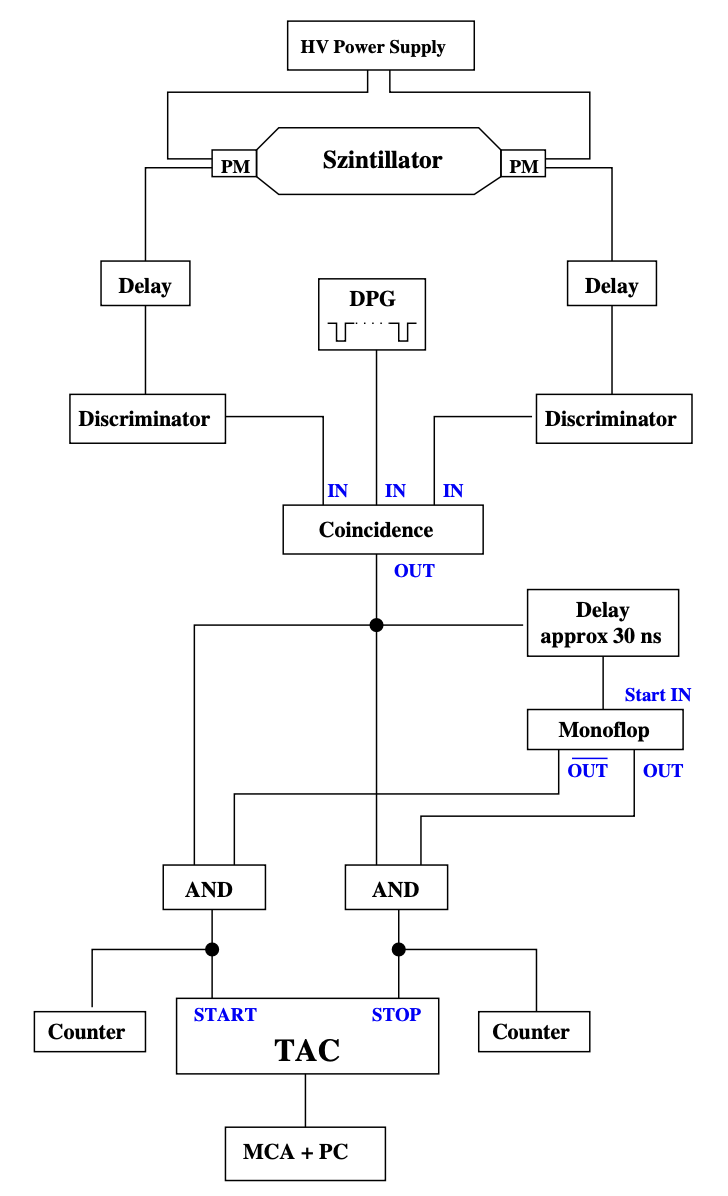
\includegraphics[width=.7\textwidth]{content/detektor.png}
    \caption{Schematische Darstellung des in dem Experiment verwendeten Detektors \cite{Anleitung01}.}
    \label{fig:detektor}
\end{figure}

\subsection{Durchführung}\label{subsec:Durchfuehrung}

Zunächst wird der Detektor aufgebaut und die Hochspannung angeschaltet.
Im ersten Messschritt wird sichergestellt, dass die Photomultiplier korrekt arbeiten, indem sie an ein Oszilloskop angeschlossen werden.
Nachdem sichergestellt wurde, dass die Photomultiplier Signale weitergeben, werden die Diskriminatoren so eingestellt, dass von beiden Photomultipliern in einer Sekunde ungefähr 30 Signale den Diskriminator verlassen.
Danach wird der Versuch zuende aufgebaut.
Die Verzögerungsleistungen werden so eingestellt, dass sich die Pulsfrequenz hinter der Koinzidenz maximiert.
Der Monoflop wird so eingestellt, dass die Suchzeit ungefähr im erwarteten Bereich der Zerfallsdauer der Myonen, also etwa $\SIrange{1}{10}{\micro\second}$, liegt.
Die TAC wird an den PC angeschlossen.\newline
Bevor die Messung gestartet werden kann, muss ein Doppelpulsgenerator verwendet und an der Koinzidenzschaltung eingeschaltet werden.
Der Doppelpulsgenerator erzeugt zwei Rechteckimpulse, die in einem festen zeitlichen Abstand zueinander liegen und von dem MCA aufgenommen werden.
Bei manuellem variieren des Abstandes der Impulse können die Kanäle des MCA kalibriert werden.
Nachdem die Kalibrierung abgeschlossen ist, wird der Doppelpulsgenerator ausgeschaltet und die Messung gestartet.
Es wird eine hinreichend lange Messzeit gewählt, um genügend Daten zu sammeln.